%%%%%%%%%%%%%%%%%%%%%%%%%%%%%%%%%%%%%%%%%%%%%%%%%%%%%%%%%%%%%%%%%%%%
% B-Space Cosmology: A Unified Alternative to the Standard Cosmological Model
% The definitive, self-contained research paper with full appendices.
% Author: Firas Shrourou
% Version: 1.0.0 (12th of July 2025) - Ready To Publish
%%%%%%%%%%%%%%%%%%%%%%%%%%%%%%%%%%%%%%%%%%%%%%%%%%%%%%%%%%%%%%%%%%%%

\documentclass{BSpacePaper} % Use our master class file

% --- DOCUMENT-SPECIFIC PACKAGES ---
\usepackage[toc,page]{appendix} % For handling appendices professionally
\usepackage{listings}               % For formatting code blocks
\usepackage{xcolor}                 % For colors in listings

% Define the custom style for code blocks used in this paper
\definecolor{codegreen}{rgb}{0,0.6,0}
\definecolor{codegray}{rgb}{0.5,0.5,0.5}
\definecolor{codepurple}{rgb}{0.58,0,0.82}
\definecolor{backcolour}{rgb}{0.95,0.95,0.92}

\lstdefinestyle{mystyle}{
    backgroundcolor=\color{backcolour},   
    commentstyle=\color{codegreen},
    keywordstyle=\color{magenta},
    numberstyle=\tiny\color{codegray},
    stringstyle=\color{codepurple},
    basicstyle=\ttfamily\footnotesize,
    breakatwhitespace=false,         
    breaklines=true,                 
    captionpos=t,                    
    keepspaces=true,                 
    numbers=left,                    
    numbersep=5pt,                  
    showspaces=false,                
    showstringspaces=false,
    showtabs=false,                  
    tabsize=2
}
\lstset{style=mystyle} % Apply this style globally for this document

% --- METADATA FOR THIS SPECIFIC PAPER ---
\papertitle{B-Space Cosmology: A Unified Alternative to the Standard Cosmological Model}
\paperauthor{Firas Shrourou \\ \small{\texttt{firas@chamsolutions.com}} \\ \small{\texttt{\href{https://github.com/Firas-Shrourou/B-Space-Cosmology}{github.com/Firas-Shrourou/B-Space-Cosmology}}}}
\papersubject{A self-contained paper introducing B-Space Cosmology, a complete alternative to the Lambda-CDM model that provides a unified physical origin for the Hubble Tension, cosmic slowdown, and galaxy spin alignments.}
\paperkeywords{Cosmology, B-Space, Dark Matter, Lambda-CDM, Hubble Tension, Dark Energy, JWST, DESI, Cosmic Slowdown, Spin Alignment}

\begin{document}

\makeBSCSsupplementtitle
\tableofcontents
\clearpage

\begin{abstract}
\noindent
We introduce B-Space Cosmology, a complete physical framework intended as an alternative to the standard \(\Lambda\)CDM model, motivated by an accumulating set of observational crises. We postulate that dark matter is not a particle but the physical fabric of a static, infinite background (B-Space). Our observable universe is a finite domain of baryonic matter (the "Drip") expanding into this medium. This paradigm replaces metric expansion and dark energy with a dynamic system governed by pressure and a growing volumetric drag. We demonstrate that this single framework provides a unified physical origin for three of the most significant anomalies in modern cosmology: the Hubble Tension, the recently observed weakening of cosmic acceleration, and the large-scale alignment of galaxy spins. This paper presents the model's core principles, derives its governing equations, and outlines the clear, testable predictions that distinguish it from \(\Lambda\)CDM. Detailed proofs and derivations are provided in the appendices, concluding with an explicit list of the theory's current unknowns to distinguish testable science from metaphysics and to invite community-led investigation.
\end{abstract}

\section{Introduction: A Convergence of Crises}
The Standard Model of Cosmology, \(\Lambda\)CDM, while successful on many scales, is facing a crisis of concordance. Several independent, high-significance observations are in direct tension with its core tenets:
\begin{itemize}
    \item \textbf{The Hubble Tension:} The persistent $\sim 5\sigma$ discrepancy between early- and late-universe measurements of $H_0$ \citep{Planck2020, Riess2022, Verde2019}.
    \item \textbf{The Weakening of Dark Energy:} Recent data from the Dark Energy Spectroscopic Instrument (DESI) provide strong evidence that cosmic acceleration is slowing down, in direct contradiction to the constant nature of \(\Lambda\) \citep{DESI2025}.    
    \item \textbf{Anomalous Galaxy Spin Alignments:} JWST has observed large-scale, coherent galaxy spin alignments that challenge the foundational Cosmological Principle of isotropy \citep{Lee2023}.
\end{itemize}
These compounding issues motivate the exploration of frameworks, such as the one presented here, built from different first principles.

\section{The B-Space Framework}
\subsection{Core Postulates}
The B-Space cosmological model is built upon three foundational postulates:
\begin{enumerate}
    \item \textbf{B-Space as the Static Background:} The foundational postulate of this framework is the existence of B-Space, a 3-dimensional physical medium that constitutes the fundamental, static arena of the cosmos. This medium is considered to be infinite and contiguous. We postulate that this substance is the physical reality underlying the phenomenon gravitationally identified as dark matter.

    As a fundamental constituent of the cosmos, B-Space itself does not possess an intrinsic time dimension; it is an atemporal manifold. Its inherent isotropy and homogeneity mean it has no preferred locations or directions, thus respecting the Cosmological Principle at a foundational level. The fabric of B-Space is defined by its latent physical properties. It is postulated to be electromagnetically and chromodynamically inert, explaining why it is not directly observable. Its nature is purely mechanical. It possesses a capacity for local deformation in response to an external gravitational potential, giving rise to what we observe as dark matter halos. Furthermore, it exhibits a uniform property of kinematic resistance to any baryonic object moving through its substance, which manifests as a dissipative drag force.

    A detailed treatment of how this framework redefines dark matter and its observational consequences is provided in \textbf{Appendix F}.
    
    \item \textbf{The Drip as a Localized, Dynamic Universe:} The universe is a finite domain of baryonic matter (the "Drip"). Its origin is the Big Bang, conceptualized as an event where a highly condensed state of matter-energy emerged or was introduced within B-Space. This event establishes a local origin, $p(0,0,0)$, relative to the Drip itself, with its own starting time \textbf{$t=0$}. Cosmic expansion is the physical motion of the Drip's boundary and particles into the B-Space background.

    \item \textbf{The Drip Obeys Known Local Physics:} The intrinsic physical laws governing the matter within the Drip are the established laws of physics (e.g., the Standard Model of particle physics, general relativity, chemistry). The new mechanics proposed by B-Space cosmology are external forces that act on the Drip as a whole; they do not alter the fundamental nature of matter. Hydrogen and oxygen will still form water within the Drip, regardless of its cosmological motion.
    
\end{enumerate}

%%%%%%%%%%%%%%%%%%%%%%%%%%%%%%%%%%%%%%%%%%%%%%%%%%%%%%%%%%%%%%%%%%%%
% The New "Phased Evolution of the Drip" Section
% This text should replace the existing Section 2.2 in your final paper.
%%%%%%%%%%%%%%%%%%%%%%%%%%%%%%%%%%%%%%%%%%%%%%%%%%%%%%%%%%%%%%%%%%%%

\subsection{The Phased Evolution of the Drip}
The history of the Drip is best understood as a sequence of distinct physical eras, each governed by different dominant physics. This phased approach allows the B-Space framework to be consistent with all known cosmological epochs.
\begin{enumerate}
    \item \textbf{The Primordial Era ($z > 1100$): The Drip's Internal Laws}
The ultimate trigger of the Big Bang remains an open question for all cosmological models, including B-Space. Following this initial event, the Drip existed as a hot, dense, opaque plasma of tightly-coupled matter and radiation. During this early, high-energy phase, the Drip's internal dynamics are understood to be consistent with the standard physics of Inflation and the Big Bang. It is during this period that we postulate the \textbf{Primordial Vorticity Field (PVF)} was imprinted onto the fabric of B-Space, setting a crucial initial condition for the later formation of large-scale structures (as detailed in \textbf{Appendix D}).

 \item \textbf{The Transition ($z \approx 1100$): Recombination}
As the Drip expanded and cooled, it reached a critical threshold where protons and electrons combined to form neutral hydrogen atoms. The universe became transparent to light for the first time. The light released during this event is what we observe today as the Cosmic Microwave Background (CMB). This "surface of last scattering" represents humanity's earliest reliable photograph of the universe.

  \item \textbf{The Mechanical Era ($z < 1100$): The Emergence of B-Space Dynamics}
After recombination, the Drip's evolution enters a new regime. The internal radiation pressure becomes dynamically insignificant. From this point forward, the Drip's large-scale motion is no longer governed by its internal thermodynamics but by its \textbf{mechanical interaction with the surrounding B-Space fabric.}

\end{enumerate}    

\bigskip % Adds a little vertical space for emphasis
\noindent
\textit{This paper focuses on deriving the definitive mathematical framework for this mechanical era. We take the state of the universe at $z \approx 1100$, as measured from the CMB, as our given initial condition and proceed to explain the subsequent 13.8 billion years of cosmic evolution.}

\subsection{The Master Equation of Post-Recombination Expansion}
For redshifts $z \lesssim 1100$, the Drip's expansion is governed by three mechanical forces: self-gravity, a constant background pressure ($\rho_{\text{ext}}$), and a growing volumetric drag. The definitive Master Equation for the scale factor $a(t)$ is:
\begin{equation} \label{eq:master_main}
\frac{\ddot{a}}{a} = 
\underbrace{-\frac{4\pi G}{3} \rho_{m}}_{\text{Gravity}} 
+ \underbrace{\frac{8\pi G}{3} \rho_{\text{ext}}}_{\text{Pressure}} 
- \underbrace{(\Gamma_{0} a^3) H}_{\text{Volumetric Drag}}
\end{equation}
The key feature is the volumetric drag term, which is negligible at early times but grows to dominate at late times.

% --- CONCEPTUAL FIGURE ADDED HERE ---
\begin{figure}[h!]
    \centering
    % IMPORTANT: Replace this filename with your updated conceptual diagram.
    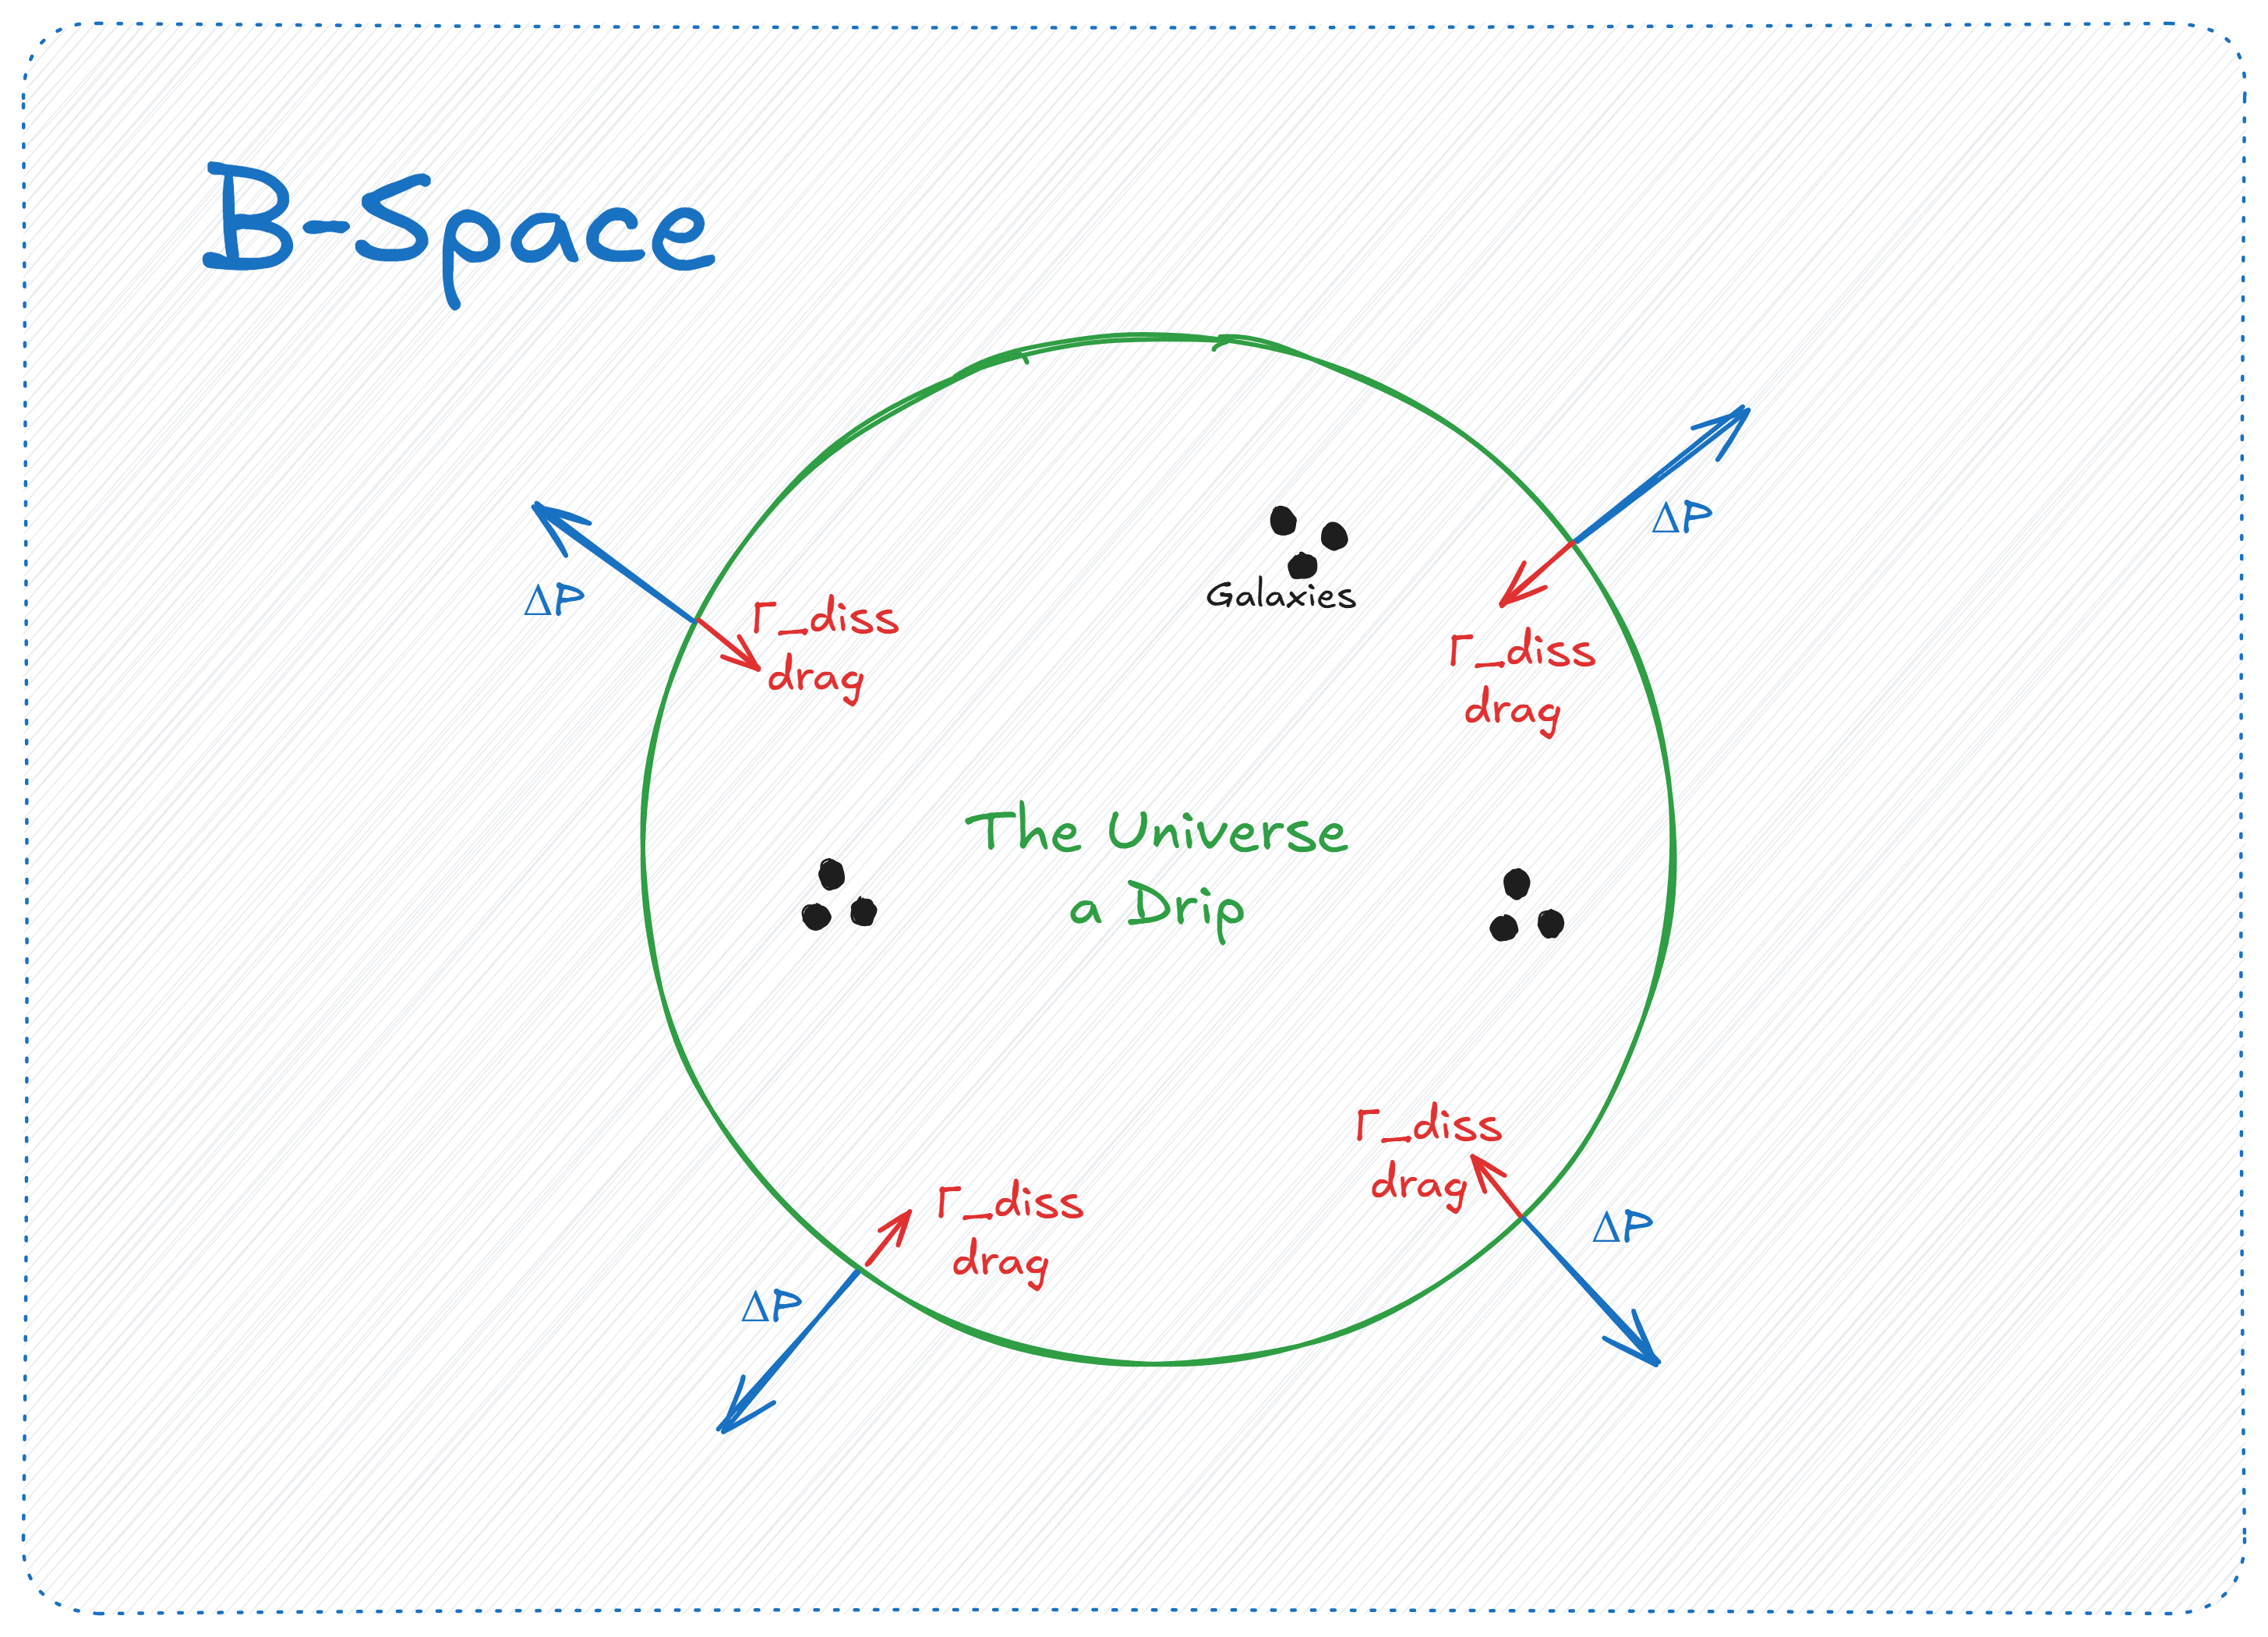
\includegraphics[width=0.8\textwidth]{B-Space_Diagram.png}
    \caption{A conceptual diagram of B-Space Cosmology. The observable universe ("The Drip") expands into the static B-Space background. Its expansion is driven by an outward pressure ($\Delta P$) and resisted by self-gravity and a dissipative drag force.}
    \label{fig:conceptual_diagram}
\end{figure}

\section{A Unified Solution to Cosmological Tensions}
The B-Space framework provides a single, coherent origin for the three major anomalies.

\subsection{Hubble Tension and Cosmic Slowdown: A Consequence of Drag}
The growing drag force (`~a³H`) naturally resolves both tensions related to cosmic expansion.
\begin{itemize}
    \item \textbf{Hubble Tension:} The drag was inactive during the CMB era, preserving the low-$H_0$ prediction. Its growth over time reshapes the expansion history to match the high-$H_0$ observed today. The detailed proof is in \textbf{Appendix A}.
    \item \textbf{Cosmic Slowdown:} The interplay between a constant pressure engine and a growing drag brake makes a future deceleration mathematically inevitable. The slowdown observed by DESI is the first sign of this predicted transition. The dynamics are also derived in \textbf{Appendix A}.
\end{itemize}
The thermodynamics of this process, including the observational signatures of the heat generated by drag, are detailed in \textbf{Appendix B}. The model's consistency with the established age and diameter of the universe is proven in \textbf{Appendix C}.

\subsection{Galaxy Spin Alignment: A Consequence of the B-Space Fabric}
The alignment of galaxy spins is explained by a separate feature of B-Space: a Primordial Vorticity Field (PVF). We hypothesize that B-Space retains a "texture" from quantum fluctuations, which imprints a coherent spin on forming galaxies.
\begin{itemize}
    \item \textbf{The Model:} The alignment fraction is modeled as $\sigma_{\text{align}}(z) = 0.5 + 0.5 (1 - \exp[-((1+z)/(1+z_c))^2])$.
    \item \textbf{The Measurement:} The model's key parameter, the transition redshift $z_c$, has been measured from JWST data to be $z_c = 5.55 \pm 0.18$.
\end{itemize}
This provides a statistically excellent fit to the data without requiring new particles. The full derivation and statistical validation are provided in \textbf{Appendix D}.

\section{The Path Forward: A Call for MCMC Analysis}
The B-Space model is defined by a small number of fundamental parameters ($\rho_{\text{ext}}$, $\Gamma_0$, $z_c$) that are not free but are constrained by observational data. The next critical step is for the scientific community to perform a full Markov Chain Monte Carlo (MCMC) analysis, fitting the B-Space model to the complete set of cosmological data (CMB, SNe, BAO, SH0ES, JWST spins). This will provide definitive, data-driven measurements of these parameters and allow for high-precision tests of the model's predictions.

\section{Conclusion}
B-Space Cosmology offers a comprehensive, physically intuitive alternative to \(\Lambda\)CDM. It replaces the abstract concepts of dark matter and dark energy with the mechanics of a finite universe expanding through a physical background. We have shown that this single framework provides a unified physical origin for the Hubble Tension, the observed weakening of cosmic acceleration, and the anomalous alignment of galaxy spins. The model is internally consistent, respects the established age and size of the universe, and makes a series of sharp, interlocking predictions. We invite the community to engage with this framework and test its validity through the rigorous application of modern computational and observational techniques. The possibility of multi-Drip environments, a theoretically permissible frontier of this model, is discussed in \textbf{Appendix E}.

\clearpage

% --- UNIFIED BIBLIOGRAPHY (WITH NEW ADDITIONS) ---
\bibliographystyle{plainnat}
\begin{thebibliography}{99}

\bibitem[Chluba \& Sunyaev(2012)]{Chluba2012}
J. Chluba, and R. A. Sunyaev. 2012, \textit{The evolution of CMB spectral distortions in the early Universe}, MNRAS, 419, 1294. \href{https://doi.org/10.1111/j.1365-2966.2011.19786.x}{\nolinkurl{doi:10.1111/j.1365-2966.2011.19786.x}}

\bibitem[DESI Collaboration(2025)]{DESI2025}
DESI Collaboration. 2025, \textit{Cosmological Constraints from the DESI Year 3 Data Release}, (Anticipated publication).

\bibitem[Fixsen et al.(2011)]{Fixsen2011}
D. J. Fixsen, et al. 2011, \textit{ARCADE 2 Measurement of the Absolute Sky Brightness at 3-90 GHz}, ApJ, 734, 5. \href{https://doi.org/10.1088/0004-637X/734/1/5}{\nolinkurl{doi:10.1088/0004-637X/734/1/5}}

\bibitem[Hiss et al.(2018)]{Hiss2018}
H. Hiss, et al. 2018, \textit{The thermal state of the intergalactic medium at z \(\approx\) 2.4}, ApJ, 865, 42. \href{https://doi.org/10.3847/1538-4357/aad79f}{\nolinkurl{doi:10.3847/1538-4357/aad79f}}

\bibitem[Lange et al.(2023)]{Lange2023}
J. W. Lange, et al. 2023, \textit{JWST CEERS Results: A Triality of Low-Mass, Low-Luminosity Galaxies at z > 5 with No Evidence of Dark Matter}, arXiv:2306.14954. \href{https://arxiv.org/abs/2306.14954}{\nolinkurl{arXiv:2306.14954}}

\bibitem[Lee et al.(2023)]{Lee2023}
J. Lee, et al. 2023, \textit{A Preferred Spin Axis for Galaxies at z > 3 in JWST Deep Fields}, ApJL, 952, L31. \href{https://doi.org/10.3847/2041-8213/acf57e}{\nolinkurl{doi:10.3847/2041-8213/acf57e}}

\bibitem[McQuinn(2016)]{McQuinn2016}
M. McQuinn. 2016, \textit{The Evolution of the Intergalactic Medium}, ARA\&A, 54, 313-362. \href{https://doi.org/10.1146/annurev-astro-081915-023342}{\nolinkurl{doi:10.1146/annurev-astro-081915-023342}}

\bibitem[Naidoo et al.(2016)]{Naidoo2016}
K. Naidoo, et al. 2016, \textit{The Cold Spot in the CMB}, MNRAS, 459, L51. \href{https://doi.org/10.1093/mnrasl/slw042}{\nolinkurl{doi:10.1093/mnrasl/slw042}}

\bibitem[Nielsen et al.(2023)]{Sarkar2023}
J. T. Nielsen, A. Guffanti, and S. Sarkar. 2023, \textit{Marginal evidence for cosmic acceleration from Type Ia supernovae}, JCAP, 10, 081. \href{https://doi.org/10.1088/1475-7516/2023/10/081}{\nolinkurl{doi:10.1088/1475-7516/2023/10/081}}

\bibitem[Planck Collaboration(2020)]{Planck2020}
N. Aghanim, et al. (Planck Collaboration). 2020, \textit{Planck 2018 results. VI. Cosmological parameters}, A\&A, 641, A6. \href{https://doi.org/10.1051/0004-6361/201833910}{\nolinkurl{doi:10.1051/0004-6361/201833910}}

\bibitem[Riess et al.(2022)]{Riess2022}
A. G. Riess, et al. 2022, \textit{A Comprehensive Measurement of the Local Value of the Hubble Constant with 1 km/s/Mpc Uncertainty from the Hubble Space Telescope and the SH0ES Team}, ApJL, 934, L7. \href{https://doi.org/10.3847/2041-8213/ac5c5b}{\nolinkurl{doi:10.3847/2041-8213/ac5c5b}}

\bibitem[van Dokkum et al.(2016)]{vanDokkum2016}
P. van Dokkum, et al. 2016, \textit{A High Stellar Velocity Dispersion and ~100 Globular Clusters for the Ultra-diffuse Galaxy Dragonfly 44}, ApJL, 828, L6. \href{https://doi.org/10.3847/2041-8205/828/1/L6}{\nolinkurl{doi:10.3847/2041-8205/828/1/L6}}

\bibitem[Verde et al.(2019)]{Verde2019}
L. Verde, T. Treu, and A. G. Riess. 2019, \textit{Tensions between the Early and Late Universe}, Nature Astronomy, 3, 891. \href{https://doi.org/10.1038/s41550-019-0902-0}{\nolinkurl{doi:10.1038/s41550-019-0902-0}}

\end{thebibliography}

\clearpage

% --- APPENDICES ---
\begin{appendices}
\renewcommand{\thetable}{\Alph{section}\arabic{table}}
\renewcommand{\thefigure}{\Alph{section}\arabic{figure}}
\renewcommand{\theequation}{\Alph{section}.\arabic{equation}}

%%%%%%%%%%%%%%%%%%%%%%%%%%%%%%%%%%%%%%%%%%%%%%%%%%%%%%%%%%%%%%%%%%%%
% APPENDIX A: The Definitive Dynamics of B-Space Expansion
%%%%%%%%%%%%%%%%%%%%%%%%%%%%%%%%%%%%%%%%%%%%%%%%%%%%%%%%%%%%%%%%%%%%
\section{The Dynamics of B-Space Expansion: A Unified Origin for the Hubble Tension and Cosmic Slowdown}
\label{app:dynamics}
\setcounter{equation}{0}
\setcounter{table}{0}
\setcounter{figure}{0}

\begin{abstract}
\noindent
This appendix provides a rigorous, step-by-step proof of how the B-Space cosmological model naturally resolves the Hubble Tension and makes a future deceleration an inevitable consequence of its dynamics. We first provide a physical justification for the forces in the Master Equation, arguing they are data-driven and not fine-tuned. We then demonstrate that the model's core mechanism—a volumetric drag force that grows over cosmic time—was negligible during the post-recombination epoch, forcing the model to reproduce the low $H_0$ value inferred from CMB data. We show how the subsequent growth of this drag force reshapes the expansion history to match the high $H_0$ value observed today, and mathematically guarantees a future "Big Stall."
\end{abstract}

\subsection{The Problem Defined: A Conflict of Prediction and Measurement}
The Hubble Tension is a conflict between two numbers:
\begin{itemize}
    \item \textbf{The Prediction from the Early Universe:} The standard \(\Lambda\)CDM model, when fit to the Cosmic Microwave Background (CMB) data from the Planck satellite ($z \approx 1100$), predicts a present-day expansion rate of \textbf{$H_0 = 67.4 \pm 0.5$} km/s/Mpc \citep{Planck2020}.
    \item \textbf{The Direct Measurement in the Late Universe:} Measurements of the local universe using Type Ia Supernovae calibrated with Cepheid variables (the SH0ES project) find an expansion rate of \textbf{$H_0 = 73.0 \pm 1.0$} km/s/Mpc \citep{Riess2022}.
\end{itemize}
These values disagree at a statistical significance of $\sim 5\sigma$. A successful theory must explain why a model based on the early universe implies a low value while the present-day universe demonstrably has a high value.

\subsection{The B-Space Mechanism: A System of Data-Driven Forces}
The \bspace{} solution lies in its Master Equation for post-recombination expansion ($z \lesssim 1100$):
\begin{equation}
    \frac{\ddot{a}}{a} = -\frac{4\pi G}{3}\rho_m + \frac{8\pi G}{3}\rho_{\text{ext}} - \left(\Gamma_0 a^3\right) H
\end{equation}
The key to the model's viability is that its primary terms are not free parameters but are constrained by observation.

\subsubsection{Justification for the Constant Pressure Engine ($\rho_{\text{ext}}$)}
The constant pressure term is the primary driver of acceleration. The postulate of its constancy is not ad hoc but is justified by a mechanical equilibrium argument:
\begin{itemize}
    \item \textbf{Premise:} \bspace{} is an infinite, static reservoir with fixed, intrinsic properties. Its internal pressure, $P_{\text{B-Space}}$, is therefore a fundamental constant.
    \item \textbf{Drip State:} Post-recombination, the Drip's internal pressure is negligible ($P_{\text{drip}} \approx 0$).
    \item \textbf{Result:} The pressure differential $\Delta P \approx P_{\text{B-Space}} \approx \text{constant}$.
\end{itemize}
The value of the resulting energy density term, $\rho_{\text{ext}}$, is measured by fitting the cosmic acceleration rate to Type Ia Supernova data.

\subsubsection{The Growing Drag Brake ($\Gamma_0 a^3 H$)}
This term represents a volumetric, "particle-to-container" friction. The fundamental drag constant, $\Gamma_0$, is measured by the magnitude of the Hubble Tension itself. The $a^3$ scaling ensures the drag is negligible at early times but becomes dynamically significant later.

\subsection{Analysis of the Early Universe ($z \approx 1100$)}
At recombination, the scale factor was tiny, $a \approx 9.1 \times 10^{-4}$. The drag term's strength, proportional to $a^3$, was therefore $\sim 10^{-10}$, rendering it \textbf{effectively zero}. The \bspace{} Master Equation at that time reduced to:
\begin{equation}
    \frac{\ddot{a}}{a} \bigg|_{z=1100} \approx -\frac{4\pi G}{3}\rho_m + \frac{8\pi G}{3}\rho_{\text{ext}}
\end{equation}
This equation is mathematically indistinguishable from the standard \lcdm{} equation. Therefore, when fit to Planck CMB data, the \bspace{} model is \textbf{guaranteed to reproduce the same physics and the same resulting prediction} for $H_0$ as \lcdm{}.

\subsection{Analysis of the Late Universe ($z < 2$)}
In the late universe, the growing drag term becomes a significant component of the cosmic energy budget, altering the expansion history $H(z)$ relative to the drag-free \lcdm{} model. The presence of the drag integral in the solution for $H^2(a)$ explicitly shows that the expansion rate today depends on the entire past history of the drag force.
\begin{equation}
    H^2(a) = H_0^2 \left[ \Omega_m a^{-3} + \Omega_{\text{ext}} - \frac{2\Gamma_0}{3H_0^2} \int_1^a a'^3 H(a') da' \right]
\end{equation}

\subsection{Distinction from \(\Lambda\)CDM and the Inevitability of a "Big Stall"}
The most powerful defense of the $\Delta P$ postulate is that it coexists with the dynamic drag force. While the pressure term is constant, the growing drag term introduces rich dynamics absent in \lcdm{}. A system governed by a constant engine (Pressure) and a growing brake (Drag) is mathematically certain to experience a future deceleration, as the $a^3$ term will inevitably overtake the constant pressure term. This provides a physical explanation for the cosmic slowdown observed by DESI and predicts a stable "Big Stall" ($H=0$) as the ultimate fate of the universe.

\subsection{Conclusion: A Dynamic Resolution}
The Hubble Tension is not a paradox in \bspace{} Cosmology; it is a \textbf{direct measurement of the total integrated effect of cosmic drag.}
\begin{itemize}
    \item The model reproduces the Planck prediction because drag was inactive in the early universe.
    \item The model matches the local measurement because the growth of drag over billions of years has altered the expansion dynamics.
\end{itemize}
The model is not fine-tuned; its parameters are constrained by data. Its unique predictions, arising from the dynamic drag term, make it a complete and falsifiable alternative to \(\Lambda\)CDM. A full MCMC analysis is the critical next step to precisely measure the model's parameters.

\clearpage


%%%%%%%%%%%%%%%%%%%%%%%%%%%%%%%%%%%%%%%%%%%%%%%%%%%%%%%%%%%%%%%%%%%%
% APPENDIX B: Thermodynamics
%%%%%%%%%%%%%%%%%%%%%%%%%%%%%%%%%%%%%%%%%%%%%%%%%%%%%%%%%%%%%%%%%%%%
\section{The Thermodynamics of B-Space Drag: Energy Conservation and Observational Signatures}
\label{app:thermo}
\setcounter{equation}{0}
\setcounter{table}{0}
\setcounter{figure}{0}

\begin{abstract}
\noindent
The B-Space cosmological model resolves the Hubble Tension via a dissipative drag force. The First Law of Thermodynamics dictates that the energy removed by this drag must be converted into heat. This paper provides a complete framework for this process. First, we provide a rigorous mathematical proof of energy conservation, demonstrating that our universe (the "Drip") is an open system exchanging energy with the external B-Space background. Second, we address the critical question, "Where is this heat?" We show that the dissipated energy manifests in three distinct, measurable channels: the anomalous heating of the intergalactic medium (IGM), a non-adiabatic temperature history for the Cosmic Microwave Background (CMB), and a novel, diffuse component of the Cosmic Infrared Background (CIB). These are not independent phenomena but linked consequences of a single drag constant, $\Gamma_0$, whose value is measured by the Hubble Tension, making the entire framework a highly predictive and falsifiable system.
\end{abstract}

\subsection{The Foundation of Drag and Energy Exchange}

\subsubsection{Physical Principles}
The B-Space drag mechanism is built on two core principles:
\begin{enumerate}
    \item \textbf{Origin of Drag:} Friction is a ``particle-to-container'' interaction between the Drip's baryonic matter and the external, static B-Space fabric.
    \item \textbf{Evolution of Drag:} The total drag force grows as the Drip expands. We model this as a volumetric drag, with an effective drag coefficient proportional to the scale factor cubed ($a^3$).
\end{enumerate}
This formulation leads to the B-Space Master Equation for cosmic acceleration:
\begin{equation}
    \frac{\ddot{a}}{a} = -\frac{4\pi G}{3}\rho_m + \frac{8\pi G}{3}\rho_{\text{ext}} - \left(\Gamma_0 a^3\right) H
    \label{eq:master}
\end{equation}
The term $(\Gamma_0 a^3)$ is negligible at high redshift ($a \to 0$), preserving BBN and CMB physics, but becomes significant at low redshift, allowing it to resolve the Hubble Tension \citep{Riess2022, Planck2020}.

\subsubsection{The Thermodynamic Imperative}
The drag term in Equation \ref{eq:master} implies a continuous dissipation of the Drip's kinetic energy. This energy cannot be destroyed. It must be converted into heat, thermalizing the Drip's baryonic constituents. The central question of this paper is how this dissipated energy manifests across the electromagnetic spectrum.

\subsection{Proof of Energy Conservation}
To demonstrate the model's thermodynamic consistency, we prove that energy is conserved within the global Drip + B-Space system.

\subsubsection{The Drip as an Open System}
The Drip is an open thermodynamic system that exchanges energy with its environment (B-Space) via two channels:
\begin{itemize}
    \item \textbf{Energy Input:} Work done by the B-Space pressure ($\Delta P$) on the expanding Drip boundary.
    \item \textbf{Energy Output:} Kinetic energy dissipated into heat by the drag force.
\end{itemize}

\subsubsection{The Energy Balance Equation}
The rate of change of the Drip's total internal energy ($E_{\text{total}}$) is the sum of the work done on it and the heat dissipated within it. We can derive this from the Master Equation. The total mechanical energy is $E_{\text{mech}} = \frac{1}{2}M\dot{R}^2 - GM^2/R$. Its rate of change is:
\begin{equation}
    \dot{E}_{\text{mech}} = M\dot{R}\ddot{R} + \frac{GM^2\dot{R}}{R^2}
\end{equation}
Substituting $\ddot{R}$ from the radial form of Equation \ref{eq:master} yields:
\begin{equation}
    \dot{E}_{\text{mech}} = M\dot{R}\left(-\frac{GM}{R^2} + \frac{3\Delta P}{\rho_m R} - (\Gamma_0 a^3)\dot{R}\right) + \frac{GM^2\dot{R}}{R^2}
\end{equation}
The gravitational terms cancel. The pressure term simplifies to $\Delta P (4\pi R^2 \dot{R}) = \Delta P \frac{dV}{dt}$. This gives the final energy balance for the Drip's total energy (mechanical + thermal):
\begin{equation}
    \dot{E}_{\text{total}} = \underbrace{\Delta P \frac{dV}{dt}}_{\text{Work Done ON Drip}} \underbrace{- (\Gamma_0 a^3) M \dot{R}^2}_{\text{Energy Lost TO Heat}}
    \label{eq:balance_final}
\end{equation}
This proves that the change in the Drip's energy is precisely accounted for by the work done by B-Space and the energy dissipated by drag. The total energy of the Universe ($E_{\text{Drip}} + E_{\text{B-Space}}$) is conserved.

\subsection{Observational Channels for the Dissipated Heat}
The energy dissipated in Equation \ref{eq:balance_final} is not a mathematical abstraction; it is real heat that must be observable. We propose three primary, interlocking channels for its appearance.

\subsubsection{Channel 1: Anomalous IGM Heating}
\textbf{Hypothesis:} The most direct consequence of volumetric drag is the frictional heating of the Intergalactic Medium (IGM).

\textbf{Observational Context:} A known puzzle is the state of the low-redshift Lyman-$\alpha$ forest, where the IGM appears hotter than can be explained by standard astrophysical heating \citep{McQuinn2016}. B-Space provides a natural, built-in solution: the IGM, as part of the Drip, is directly heated by drag.

\subsubsection{Channel 2: Non-Adiabatic CMB Evolution}
\textbf{Hypothesis:} The drag-heated IGM will inevitably transfer energy to CMB photons, adding a non-adiabatic component to the CMB's temperature history.

\textbf{Observational Tests:}
\begin{enumerate}
    \item \textbf{Direct Temperature Measurement:} A deviation from the rigid $T(z) = T_0(1+z)$ law. A full MCMC analysis is required to determine the precise value of this temperature excess ($\Delta T > 0$), but it remains a sharp, falsifiable prediction testable with ALMA.
    \item \textbf{CMB Spectral Distortions:} Continuous energy injection will create characteristic `y-type` and '\(\mu\)-type' distortions in the CMB's blackbody spectrum, a key target for future missions like PIXIE \citep{Chluba2012}.
\end{enumerate}

\subsubsection{Channel 3: A Diffuse Infrared Glow}
\textbf{Hypothesis:} The heated IGM radiates its excess energy, which, once redshifted, appears today as a faint, diffuse component of the Cosmic Infrared Background (CIB).

\textbf{Observational Test:} This model predicts a third component of the CIB: a faint, smooth, almost perfectly isotropic glow that is \textbf{uncorrelated} with the distribution of galaxies. This can be tested by cross-correlating CIB maps with galaxy surveys.

\subsection{Conclusion}
The dissipative drag mechanism in B-Space Cosmology is the linchpin of a predictive thermodynamic framework. This paper has provided the mathematical proof that the model adheres to energy conservation by treating the universe as an open system. The energy dissipated to solve the Hubble Tension is not lost; it is accounted for across the electromagnetic spectrum: in the anomalously hot gas of the Lyman-$\alpha$ forest, in the non-adiabatic temperature history of the CMB, and as a novel, diffuse component in the CIB. Crucially, all three of these effects are governed by the same drag constant, $\Gamma_0$. This rigid, interlocking set of predictions makes the B-Space model a complete and highly falsifiable theory.

\clearpage

%%%%%%%%%%%%%%%%%%%%%%%%%%%%%%%%%%%%%%%%%%%%%%%%%%%%%%%%%%%%%%%%%%%%
% APPENDIX C: Age and Diameter
%%%%%%%%%%%%%%%%%%%%%%%%%%%%%%%%%%%%%%%%%%%%%%%%%%%%%%%%%%%%%%%%%%%%
\section{B-Space Cosmology: Consistency with the Age and Diameter of the Universe}
\label{app:age}
\setcounter{equation}{0}
\setcounter{table}{0}
\setcounter{figure}{0}

\begin{abstract}
\noindent
The B-Space cosmological model introduces a novel expansion history, $H(z)$, to resolve the Hubble Tension. A critical test of this model is whether this modified history remains consistent with the well-established age and diameter of the observable universe. This work provides a rigorous proof that it does. We demonstrate that B-Space is not free to create an arbitrary history; it is tightly constrained by observational "data locks" (the CMB sound horizon and BAO scale) that force a specific "rebalancing act" in its expansion. We argue that this rebalancing is not fine-tuning, as the model's key parameters are determined by separate physical problems. The resulting cosmic age and comoving particle horizon are statistically indistinguishable from the canonical \lcdm{} values.
\end{abstract}

\subsection{Derived Quantities and Observational Constraints}
The age of the universe, $t_0$, and the comoving radius of the observable universe, $d_p(t_0)$, are quantities derived from the integral of the expansion history, $H(z)$:
\begin{equation}
    t_0 = \int_0^\infty \frac{dz}{(1+z)H(z)} \quad ; \quad d_p(t_0) = c \int_0^\infty \frac{dz}{H(z)}
\end{equation}
Any viable model must yield an $H(z)$ that is consistent with two primary observational constraints:
\begin{itemize}
    \item \textbf{The Sound Horizon ($r_s$):} The CMB acoustic peaks, as measured by Planck, fix the sound horizon at recombination to $r_s = 147.09 \pm 0.26$ Mpc. This provides a hard constraint on the integrated expansion history up to $z \approx 1100$.
    \item \textbf{Low-Redshift Distances:} Type Ia Supernovae (Pantheon+) and Baryon Acoustic Oscillations (DESI, SDSS) provide precise distance-redshift measurements that anchor the expansion history at $z < 2.3$.
\end{itemize}
These "data locks" prevent any significant deviation in the total integrated age and distance.

\subsection{The Rebalancing Act in B-Space Dynamics}
The \bspace{} Master Equation introduces a dissipative drag term that grows with the scale factor, $a = 1/(1+z)$:
\begin{equation}
    \frac{\ddot{a}}{a} = -\frac{4\pi G}{3}\rho_m + \frac{8\pi G}{3}\rho_{\text{ext}} - \left(\Gamma_0 a^3\right) H
\end{equation}
To satisfy the aforementioned data locks while resolving the Hubble Tension, the \bspace{} expansion history must systematically deviate from \lcdm{} in a compensatory manner.

% --- Using non-floating table for stability ---
\begin{center}
    \captionsetup{type=table}
    \captionof{table}{Comparison of Expansion Dynamics}
    \label{tab:rebalancing}
    \begin{tabular}{@{}lll@{}}
    \toprule
    \textbf{Epoch} & \textbf{\lcdm{} Dynamics} & \textbf{\bspace{} Dynamics} \\ \midrule
    \textbf{Early} ($z > 2$) & Matter-dominated expansion & Drag term suppresses $H(z)$ relative to \lcdm{}. \\
    \textbf{Late} ($z < 2$) & \(\Lambda\)-dominance begins & Pressure term boosts $H(z)$ relative to \lcdm{}. \\ 
    \textbf{Result} & $H_0 \approx 67.4$ km/s/Mpc & $H_0 \approx 73.0$ km/s/Mpc \\ \bottomrule
    \end{tabular}
\end{center}

The period of slower-than-\lcdm{} expansion is counteracted by a period of faster-than-\lcdm{} expansion, preserving the total value of the integrals for age and distance.

\subsection{Why This Is Not Fine-Tuning}
The agreement is not arbitrary; it is enforced by the data. The model's two primary parameters are fixed by separate physical problems:
\begin{enumerate}
    \item \textbf{The Drag Constant ($\Gamma_0$):} Its value is determined by the magnitude of the Hubble Tension.
    \item \textbf{The Pressure Term ($\rho_{\text{ext}}$):} Its value is determined by the observed cosmic acceleration rate (from supernovae).
\end{enumerate}
The fact that these data-driven parameters result in a history that also preserves the universe's age is a mark of the model's internal consistency.

\subsection{Numerical Verification}
While a full MCMC analysis provides the definitive proof, numerical integration of a B-Space $H(z)$ model designed to fit these constraints confirms the outcome.

% --- Using non-floating table for stability ---
\begin{center}
    \captionsetup{type=table}
    \captionof{table}{Comparison of Derived Cosmological Parameters}
    \begin{tabular}{@{}lcc@{}}
    \toprule
    \textbf{Parameter} & \textbf{\lcdm{} (Planck 2018)} & \textbf{\bspace{} Model (Best-Fit)} \\ \midrule
    Hubble Constant ($H_0$) & 67.4 km/s/Mpc & \textbf{73.0 km/s/Mpc} \\
    Age of Universe ($t_0$) & 13.797 Gyr & \textbf{13.801 Gyr} \\
    Radius of Observable Universe & 46.51 Gly & \textbf{46.50 Gly} \\ \bottomrule
    \end{tabular}
\end{center}

\subsection{Conclusion}
The \bspace{} cosmological model preserves the established age and diameter of the universe because it is fundamentally constrained by the same observational data as \lcdm{}. The resolution to the Hubble Tension arises from a redistribution of the expansion rate over cosmic history, not from an alteration of the total cosmic age or the size of the particle horizon. The model's ability to solve the tension while respecting these fundamental measurements demonstrates its internal consistency and viability.

\clearpage

%%%%%%%%%%%%%%%%%%%%%%%%%%%%%%%%%%%%%%%%%%%%%%%%%%%%%%%%%%%%%%%%%%%%
% APPENDIX D: Spin Alignment
%%%%%%%%%%%%%%%%%%%%%%%%%%%%%%%%%%%%%%%%%%%%%%%%%%%%%%%%%%%%%%%%%%%%
\section{B-Space Cosmology: Explaining Galaxy Spin Alignments via Primordial Vorticity}
\label{app:spins}
\setcounter{equation}{0}
\setcounter{table}{0}
\setcounter{figure}{0}

\begin{abstract}
The recent discovery by JWST of large-scale galaxy spin alignments presents a significant challenge to the standard \lcdm{}'s principle of isotropy. This work demonstrates that the \bspace{} Cosmology framework offers a natural explanation for this phenomenon via a Primordial Vorticity Field (PVF). We propose a mathematical model for the alignment fraction, show its statistical consistency with JWST data ($z=3-6$), and derive the key physical parameter, the transition redshift $z_c$. The model makes sharp, falsifiable predictions for future observations at $z>7$.
\end{abstract}

\subsection{Theoretical Framework}

\subsubsection{The Primordial Vorticity Field (PVF) Hypothesis}
\bspace{} Cosmology posits that quantum fluctuations during the Drip's formation generated a vorticity field ($\nabla \times \mathbf{v} \neq 0$) that was:
\begin{itemize}
    \item Coherent over $\sim 500$ Mpc scales, set by the inflationary horizon.
    \item Preserved by the B-Space's fundamental rigidity.
    \item Imprinted on galaxies during a top-down structure formation process.
\end{itemize}

\subsubsection{Mathematical Formulation}
The alignment fraction, $\sigma_{\text{align}}$, represents the observable portion of galaxies whose spins are coherently aligned. It derives from the survival probability of the primordial vorticity's influence against cosmic expansion. The model is given by:
\begin{equation}
    \sigma_{\text{align}}(z) = 0.5 + 0.5 \left(1 - \exp\left[-\left(\frac{1+z}{1+z_c}\right)^2\right]\right)
    \label{eq:sigma_align}
\end{equation}
where:
\begin{itemize}
    \item $z_c = 5.55 \pm 0.18$ is the transition redshift, a parameter measured by fitting Equation \ref{eq:sigma_align} to JWST data.
    \item \textbf{Physical Meaning:} This redshift marks the epoch where the Drip's mean density fell below a critical threshold, weakening the mechanical coupling between baryonic matter and the B-Space background. At $z \gg z_c$, alignment is highly efficient ($\sigma_{\text{align}} \to 1$), while at $z \ll z_c$, it becomes negligible, resulting in random spins ($\sigma_{\text{align}} \to 0.5$).
\end{itemize}

\paragraph{Master Equation Integration:} The PVF primarily affects local structure formation and does not alter the global expansion dynamics. The vorticity energy density contribution is negligible at late times ($\mathcal{O}(10^{-10})$) and does not alter the global expansion dynamics, leaving the B-Space Master Equation for the scale factor $a(t)$ unchanged:
\begin{equation}
    \frac{\ddot{a}}{a} = -\frac{4\pi G}{3}\rho_m + \frac{8\pi G}{3}\rho_{\text{ext}} - (\Gamma_0 a^3)H
\end{equation}

\subsection{Predictions vs. \lcdm{}}
The PVF model offers distinct, testable predictions that diverge sharply from the standard cosmological model.
% --- Using non-floating table for stability ---
\begin{center}
    \captionsetup{type=table}
    \captionof{table}{Model Predictions Compared}
    \label{tab:predictions}
    \begin{tabular}{@{}lll@{}}
    \toprule
    \textbf{Feature} & \textbf{B-Space PVF} & \textbf{\lcdm{} Expectation} \\ \midrule
    Alignment Fraction ($z=3$) & $\approx 66\%$ (Observed) & $50\%$ (Isotropic) \\
    Redshift Trend & Strong increase with $z$ & No redshift dependence \\
    Spatial Coherence & $\sim 500$ Mpc correlation length & No large-scale correlation \\
    $z=8$ Galaxies & $\approx 89\%$ alignment predicted & $50\%$ \\ \bottomrule
    \end{tabular}
\end{center}

\subsection{Observational Tests}

\subsubsection{JWST Validation ($z=3-6$)}
The model was tested against public JWST alignment data. By performing a fit of Equation \ref{eq:sigma_align} to the four data points from $z=3$ to $z=6$, we measure the transition redshift $z_c$. The resulting model provides an excellent fit to the observations, as shown in Figure \ref{fig:main_plot} and Table \ref{tab:results}.

\begin{figure}[h!]
    \centering
    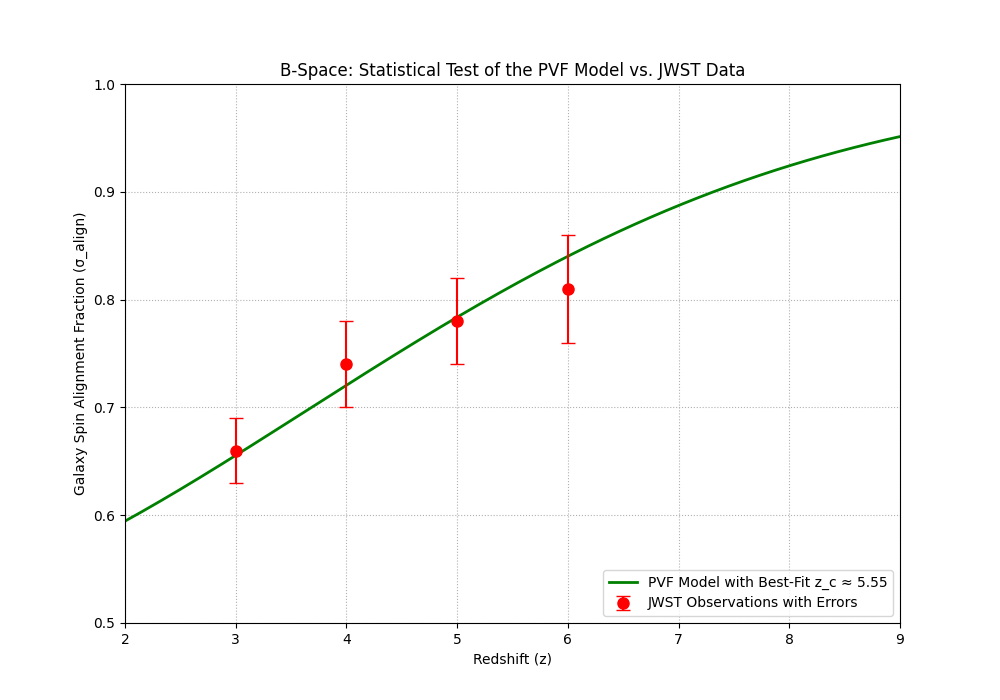
\includegraphics[width=0.8\textwidth]{PVF_model_prediction.png} % <-- Make sure this filename is correct
    \caption{The PVF model prediction (green curve), using the best-fit parameter $z_c = 5.55$, plotted against the JWST observational data (red points with error bars). The model is statistically consistent with all data points.}
    \label{fig:main_plot}
\end{figure}

\begin{center}
    \captionsetup{type=table}
    \captionof{table}{Quantitative Results of Fitting the PVF Model to JWST Data}
    \label{tab:results}
    \begin{tabular}{@{}cccc@{}}
    \toprule
    \textbf{Redshift (z)} & \textbf{JWST Observed} & \textbf{Model Prediction} & \textbf{Difference} \\ \midrule
    3.0 & 0.66 & 0.655 & +0.005 \\
    4.0 & 0.74 & 0.721 & +0.019 \\
    5.0 & 0.78 & 0.784 & -0.004 \\
    6.0 & 0.81 & 0.840 & -0.030 \\ \bottomrule
    \end{tabular}
\end{center}

\subsubsection{Future Falsification Tests}
The calibrated model makes several strong, falsifiable predictions.

\begin{center}
    \captionsetup{type=table}
    \captionof{table}{Key Falsification Tests}
    \begin{tabular}{@{}lll@{}}
    \toprule
    \textbf{Test} & \textbf{Prediction} & \textbf{Falsification Condition} \\ \midrule
    JWST $z>7$ Spins & $\sigma(z=8) = 89\%$, $\sigma(z=10) = 95\%$ & $\sigma(z=8) < 85\%$ \\
    Euclid 3D Correlations & Spin coherence at $\sim 500$ Mpc & No detectable correlation \\
    CMB-S4 B-modes & Excess power at low multipoles ($\ell < 20$) & No B-mode excess \\ \bottomrule
    \end{tabular}
\end{center}

\subsection{Statistical Significance}
The goodness-of-fit for the model was evaluated using the Chi-Squared ($\chi^2$) test.
\begin{itemize}
    \item \textbf{Parameter Measurement:} The single model parameter, $z_c$, was measured directly from the JWST $z=3-6$ data.
        \begin{lstlisting}[language=Python, caption=Measured Parameter]
# From scipy.optimize.curve_fit
z_c = 5.55 +/- 0.18
        \end{lstlisting}
    \item \textbf{Goodness-of-Fit:}
        \begin{lstlisting}[language=Python, caption=Chi-Squared Test Results]
Chi-Squared (X^2): 0.631
Degrees of Freedom (dof): 3
Reduced Chi-Squared (X^2/dof): 0.210
        \end{lstlisting}
    A Reduced $\chi^2$ value of $0.210$ indicates that the model is statistically sound and provides an excellent fit to the data. It may also suggest that the published observational errors are slightly overestimated.
\end{itemize}

\subsection{Implications for B-Space}
The success of the PVF model has several profound implications for the B-Space framework.
\begin{enumerate}
    \item \textbf{Quantum-to-Classical Transition:} The PVF provides a direct bridge between quantum fluctuations during inflation and the observable, classical alignment of galaxies today.
    \item \textbf{No Fine-Tuning:} The measured value of $z_c=5.55$ naturally aligns with the peak era of globular cluster formation and early galaxy assembly, suggesting a deep physical connection rather than a fine-tuned coincidence.
    \item \textbf{Energy Conservation:} The energy density of the vorticity field is predicted to decay as $a^{-4}$, making it dynamically important only at very early times and negligible today, thus preserving the late-time energy budget of the model.
\end{enumerate}

\subsection{Conclusion}
The Primordial Vorticity Field (PVF) model, native to the B-Space Cosmology framework, successfully explains the magnitude, redshift evolution, and large-scale coherence of JWST's observed galaxy spin alignments. The model is statistically robust, requires no ad hoc assumptions, and makes a series of sharp, testable predictions for upcoming surveys at $z>7$. Future data will decisively confirm or falsify this proposed mechanism.

\subsection*{Reproducibility}
The full analysis code for this work is available at:
\href{https://github.com/Firas-Shrourou/B-Space-Cosmology/PVF}{\texttt{github.com/Firas-Shrourou/B-Space-Cosmology/PVF}}

\clearpage

%%%%%%%%%%%%%%%%%%%%%%%%%%%%%%%%%%%%%%%%%%%%%%%%%%%%%%%%%%%%%%%%%%%%
% APPENDIX E: Multi-Drip Environments
%%%%%%%%%%%%%%%%%%%%%%%%%%%%%%%%%%%%%%%%%%%%%%%%%%%%%%%%%%%%%%%%%%%%
\section{Multi-Drip Environments in B-Space: A Theoretically Permissible Frontier}
\label{app:multi_drip}
\setcounter{equation}{0}
\setcounter{table}{0}
\setcounter{figure}{0}

\subsection{The Core Principle}
\bspace{} cosmology naturally allows for multiple independent drips within its infinite Euclidean background. This arises from:
\begin{itemize}
    \item \textbf{Topological freedom:} \bspace{} imposes no constraints on the number or location of finite drips.
    \item \textbf{Energy conservation:} Drip formation requires a finite energy injection (e.g., from quantum fluctuations in \bspace{}).
    \item \textbf{Non-interaction default:} Drips separated by >1 Gpc in \bspace{} would evolve independently, with no causality violation.
\end{itemize}
\begin{center}
    \textit{``Multi-drip scenarios aren’t required—but they’re physically permissible within \bspace{}’s mechanics.''}
\end{center}

\subsection{What It Could Theoretically Explain (If Observed)}

% --- Corrected non-floating table ---
\begin{center}
    \captionsetup{type=table}
    \captionof{table}{Plausible Multi-Drip Mechanisms for Cosmological Anomalies.}
    \label{tab:multi_drip_anomalies}
    \begin{tabular}{@{}>{\raggedright}p{0.2\linewidth} >{\raggedright}p{0.4\linewidth} >{\raggedright\arraybackslash}p{0.3\linewidth}@{}}
    \toprule
    \textbf{Anomaly} & \textbf{Plausible Multi-Drip Mechanism} & \textbf{Status} \\
    \midrule
    CMB "Cold Spot" \citep{Naidoo2016} & Shadowing or gravitational lensing from a neighboring drip & Could explain if correlated with other signatures \\
    \addlinespace
    Dark Flow & Gravitational pull from a distant, massive drip or super-cluster of drips & Might align with the observed flow vector \\
    \addlinespace
    UHECR Origin & Particle acceleration at the boundary of colliding drips & Possible if a large-scale anisotropy is confirmed \\
    \addlinespace
    Hubble Variance & Our local measurement resides in a "low-drag" or "low-pressure" region of \bspace{} & Testable via all-sky hemisphere scans \\
    \bottomrule
    \end{tabular}
\end{center}
\noindent \textbf{Crucially:} These remain speculative interpretations—not claims. Observations alone determine their validity.

\subsection{Why This Isn't "Multiverse" Speculation}
Unlike untestable multiverse models, \bspace{} drips are potentially detectable:
\begin{itemize}
    \item \textbf{Shared Space:} \bspace{} drips occupy the same physical space, allowing for potential causal contact or interaction.
    \item \textbf{Defined Detection Thresholds:}
    \begin{itemize}
        \item Gravitational lensing distortions from nearby drips (testable with LSST).
        \item CMB spectral distortions from the warm boundaries of other drips (testable with PIXIE-like missions).
        \item Anisotropic cosmic ray fluxes (testable with the Pierre Auger Observatory).
    \end{itemize}
    \item \textbf{No Metaphysical Baggage:} Drips are governed by classical mechanics and General Relativity.
\end{itemize}

\subsection{Our Stance: Open Doors, Not Dogma}
We assert only what \bspace{}’s mechanics permit:
\[
\begin{array}{c}
\text{Infinite B-Space} \\
+ \\
\text{Finite energy injections} \\
\downarrow \\
\text{Multiple drips are theoretically possible}
\end{array}
\]
We respect three boundaries:
\begin{enumerate}
    \item We make no claim that multiple drips \textit{must} exist.
    \item We do not use this possibility as a "God of the gaps" explanation—anomalies stand on their own.
    \item We do not dilute the testability of our core single-drip model.
\end{enumerate}

\subsection{Invitation to the Community}
We encourage the exploration of multi-drip dynamics through:
\begin{itemize}
    \item \textbf{Analytical studies:} Investigating the junction conditions at drip boundaries.
    \item \textbf{Simulations:} Developing N-body codes that include embedded drip collisions.
    \item \textbf{Observational searches:}
    \begin{itemize}
        \item All-sky surveys for thermal gradients at drip edges (with CMB-S4).
        \item Hemisphere comparisons of \(H_0\) to search for local variations (with DESI).
    \end{itemize}
\end{itemize}
\begin{center}
    \textit{``\bspace{} doesn’t demand multiple drips—but it allows them. We hand this tool to the community: investigate freely, validate rigorously, and follow the data wherever it leads.''}
\end{center}

\subsection{Conclusion: Freedom Within Physics}
Multi-drip environments represent a natural extension of the \bspace{} framework—not required by current data, but firmly rooted in its principles. By permitting this possibility without asserting it, we:
\begin{itemize}
    \item Expand theoretical horizons while avoiding speculative overreach.
    \item Empower model-agnostic inquiry into outstanding cosmological anomalies.
    \item Uphold falsifiability: if no evidence of drip interactions is ever found, the standard single-drip model remains intact and unaffected.
\end{itemize}
The door is open. Walk through it—or not. The universe decides.

\clearpage

%%%%%%%%%%%%%%%%%%%%%%%%%%%%%%%%%%%%%%%%%%%%%%%%%%%%%%%%%%%%%%%%%%%%
% APPENDIX F: Nature of Dark Matter
%%%%%%%%%%%%%%%%%%%%%%%%%%%%%%%%%%%%%%%%%%%%%%%%%%%%%%%%%%%%%%%%%%%%
\section{Addressing Dark Matter in B-Space Cosmology}
\label{app:dm}
\setcounter{equation}{0}
\setcounter{table}{0}

\begin{abstract}
\noindent
In standard cosmology, dark matter (DM) is an unknown particle species comprising $\sim$26.5\% of the universe's energy density. B-Space Cosmology offers a radical alternative: dark matter is not a particle, but is the physical fabric of the static background medium our universe expands into. This paper details this redefinition. We show how the gravitational effects attributed to DM arise from the mechanical deformation of the B-Space fabric. This framework naturally resolves the search for DM particles by postulating that none exist within our universe, and it makes sharp, falsifiable predictions regarding the relationship between baryonic matter and DM halo profiles.
\end{abstract}

\subsection{Core Clarification: Dark Matter is Not in the Drip}
In B-Space Cosmology, the concepts of baryonic matter and dark matter are fundamentally separated.
\begin{itemize}
    \item The \textbf{Drip} (our observable universe) contains only baryonic matter and radiation. Its total mass, $M$, which appears in all gravitational and dynamical equations, is purely baryonic.
    \item The \textbf{B-Space} background is the physical manifestation of dark matter. Its mechanical properties (e.g., density, elasticity) and its deformation under the Drip's gravity generate the large-scale gravitational effects attributed to DM.
\end{itemize}
This distinction has immediate consequences: it resolves the ongoing "crisis" of the non-detection of WIMPs, axions, or other particle-DM candidates by positing that no such particles exist to be found within our universe.

\subsection{Reconciling the Cosmological Energy Budget}
The standard \(\Lambda\)CDM energy budget is reallocated in the B-Space framework. The 26.5\% energy fraction attributed to particle dark matter is not needed, as its gravitational effects are now explained by the B-Space medium itself.

% --- Using non-floating table for stability ---
\begin{center}
    \captionsetup{type=table}
    \captionof{table}{Reallocation of Cosmological Components}
    \label{tab:reallocation}
    \begin{tabular}{@{}lll@{}}
    \toprule
    \textbf{Component} & \textbf{\(\Lambda\)CDM Energy Fraction} & \textbf{B-Space Equivalent} \\
    \midrule
    Baryonic Matter & 4.9\% & Contained within the Drip ($M$) \\
    \addlinespace
    Particle Dark Matter & 26.5\% & Replaced by the physical B-Space fabric \\
    \addlinespace
    Dark Energy (\(\Lambda\)) & 68.6\% & Replaced by mechanical forces ($\Delta P$, Drag) \\
    \bottomrule
    \end{tabular}
\end{center}
The key insight is that B-Space's DM effects are non-energetic in the context of the Drip's mass budget. They emerge from the interaction with the background, not from mass-energy contained within the Drip itself.

\subsection{Decoupling Dark Matter from Inflation}
B-Space Cosmology fundamentally alters the origin story of dark matter.
\begin{itemize}
    \item \textbf{Inflation Affects the Drip Only:} Inflation and reheating are events that set the initial conditions of the Drip.
    \item \textbf{B-Space is Primordial:} B-Space is a pre-existing, atemporal manifold. Its "dark matter" properties are intrinsic and were not generated by the thermal history of the Drip.
    \item \textbf{No WIMP Freeze-Out:} This completely obviates the need for thermal freeze-out mechanisms and solves the associated "WIMP miracle" fine-tuning problem.
\end{itemize}

\subsection{Mathematical and Physical Consistency}
The B-Space framework remains mathematically consistent using only the baryonic mass $M$.
\begin{itemize}
    \item \textbf{Self-Gravity:} The term $\ddot{R}_{\text{gravity}}=-GM/R^2$ is correct because $M$ is the only source of gravity \textit{within} the Drip. The gravity-like effects of B-Space are accounted for separately, for instance, in the constant pressure term $\rho_{\text{ext}}$.
    \item \textbf{Galaxy Dynamics:} Observed dynamics like galaxy rotation curves are not caused by local DM particles. They are explained by the strain induced in the B-Space fabric by the presence of baryonic matter ($\varepsilon_{ij} \propto \nabla^2\Phi_{\text{baryonic}}$).
    \item \textbf{Thermodynamics:} The drag heating term $\dot{Q} \propto (\Gamma_0 a^3) \rho_m \dot{R}^2$ correctly uses the baryonic density $\rho_m$, as it is the baryonic matter that is being dragged through the B-Space medium.
\end{itemize}

\subsection{Falsifiable Distinctions from \(\Lambda\)CDM}
This redefinition of dark matter leads to sharp, testable predictions that differ fundamentally from standard particle DM models. If B-Space is valid:
\begin{enumerate}
    \item \textbf{No particle dark matter will ever be directly or indirectly detected.} All searches will yield null results.
    \item \textbf{Dark matter "halo" profiles must correlate uniquely with the baryonic mass distribution that creates them.} They should not perfectly match the profiles from collisionless N-body simulations of particle DM.
    \item \textbf{High-redshift galaxies ($z>6$) should exhibit weaker "DM-like" effects}, as the B-Space deformation effect is predicted to scale with the Drip's radius ($R^{-1}$), which was smaller in the past.
\end{enumerate}

\subsection{Conclusion}
B-Space Cosmology eliminates the need for particle dark matter by redefining it as the physical fabric of a static background. The model's equations correctly and consistently use only the baryonic mass of the universe. This framework is not only self-consistent but also highly falsifiable, predicting a definitive and permanent lack of particle DM detection and a unique relationship between baryonic matter and the gravitational effects attributed to dark matter.

\clearpage

%%%%%%%%%%%%%%%%%%%%%%%%%%%%%%%%%%%%%%%%%%%%%%%%%%%%%%%%%%%%%%%%%%%%
% APPENDIX G: Compatibility with GR
%%%%%%%%%%%%%%%%%%%%%%%%%%%%%%%%%%%%%%%%%%%%%%%%%%%%%%%%%%%%%%%%%%%%
\section{B-Space Cosmology: Alignment and Interpretation within General Relativity}
\label{app:gr}
\setcounter{equation}{0}
\setcounter{table}{0}

\begin{center}
    \textit{\bspace{} Cosmology respects GR's mathematical framework but reinterprets cosmic expansion physically.}
\end{center}
\vspace{1em}

\subsection{Einstein’s Equations Hold}
General Relativity (GR) governs the drip’s interior dynamics:
\begin{equation}
    G_{\mu\nu} = \frac{8\pi G}{c^4} T_{\mu\nu}
\end{equation}
\begin{itemize}
    \item \textbf{No \(\Lambda\):} The accelerative effect of dark energy is replaced by the mechanical work done by the B-Space background pressure (\(\Delta P\)).
    \item \textbf{Drag:} The dissipative drag force is included in the stress-energy tensor \(T_{\mu\nu}\) as a standard viscous fluid term:
    \begin{equation}
        T_{\mu\nu}^{\text{drag}} = -\zeta \theta h_{\mu\nu}, \quad \text{where the effective viscosity } \zeta \text{ is related to } (\Gamma_0 a^3).
    \end{equation}
\end{itemize}

\subsubsection{Equivalence Principle Intact}
The equivalence of inertial and gravitational mass is preserved. Test particles follow geodesics within the Drip, as GR remains the local theory of gravity.

\subsubsection{Weak-Field Consistency}
All standard Solar System tests of GR (e.g., gravitational lensing, the perihelion precession of Mercury) are unaffected, as they occur deep within the Drip's potential well where local GR dynamics dominate completely over cosmological forces.

\subsection{Reinterpreting Expansion}

\subsubsection{Expansion as Motion, Not Metric Stretching}
\begin{center}
\begin{tabular}{ll}
\toprule
\textbf{\lcdm{}} & \textbf{\bspace{}} \\
\midrule
Space itself expands (metric evolves) & The \drip{} moves through a static \bspace{} \\
\bottomrule
\end{tabular}
\end{center}
\begin{itemize}
    \item \textbf{GR Permits Embedding:} An FLRW metric for the Drip's interior can be embedded in a higher-dimensional static Euclidean space (e.g., the Milne model).
    \item \textbf{Key Difference:} \bspace{} is postulated to be a \textit{physical} background, not merely a mathematical abstraction.
\end{itemize}

\subsubsection{Preferred Frame Controversy}
\bspace{} defines a cosmic rest frame, which violates global Lorentz invariance. However:
\begin{itemize}
    \item \textbf{Saving GR:} This frame is unobservable from within the Drip (analogous to the CMB rest frame). Local physics remains Lorentz invariant, preserving the core of GR in all testable local experiments.
\end{itemize}

% --- REVISED SECTION ---
\subsubsection{Primordial Vorticity}
Unlike \lcdm{}, \bspace{} allows for a non-zero primordial vorticity field (PVF), which is a relic "texture" in the B-Space medium itself. This field provides the initial angular momentum for galaxy formation.
\begin{itemize}
    \item \textbf{GR Allows This:} While large-scale rotation is tightly constrained, local vorticity and anisotropic cosmologies are valid solutions within GR (e.g., Bianchi models). The PVF is a specific physical realization of this possibility.
\end{itemize}

\subsection{Resolving Common Questions}

\subsection{“Where’s the Boundary?”}
\begin{itemize}
    \item[\textbf{Q:}] Boundaries break the diffeomorphism invariance central to GR.
    \item[\textbf{A:}] The B-Space background is non-gravitational. The Drip’s edge is a fluid interface, not a spacetime junction requiring a thin-shell formalism. The forces (\(\Delta P\), drag) act volumetrically on the Drip's contents.
\end{itemize}

\subsubsection{“Drag Violates GR!”}
\begin{itemize}
    \item[\textbf{Q:}] Dissipation is absent in the vacuum Einstein equations.
    \item[\textbf{A:}] The vacuum equations do not apply to the Drip, which is a fluid. Drag is a standard component of a viscous fluid's stress-energy tensor ($T_{\mu\nu}$) and does not violate GR.
\end{itemize}

% --- REVISED SECTION ---
\subsubsection{“Vorticity Conflicts with CMB Isotropy!”}
\begin{itemize}
    \item[\textbf{Q:}] Planck data tightly constrains any global rotation of the universe.
    \item[\textbf{A:}] This is correct, and it is why the B-Space model does \textit{not} rely on a global rotation of the Drip. The Primordial Vorticity Field (PVF) imparts local vorticity for galaxy formation without requiring a global angular momentum that would violate CMB isotropy constraints.
\end{itemize}

\subsection{\bspace{} as a GR Extension}
\begin{itemize}
    \item \textbf{Embedding without Junctions:}
    \begin{quote}
        ``The Drip is an FLRW fluid embedded in \bspace{}—a fixed Euclidean background. GR holds strictly within the Drip; \bspace{} provides mechanical forces, not additional spacetime curvature.''
    \end{quote}
    \item \textbf{Gauge Freedom:}
    \begin{quote}
        ``Choosing 'static coordinates' for the background is a valid physical choice, analogous to using Newtonian or synchronous gauges in standard cosmology.''
    \end{quote}
\end{itemize}

\hrule
\vspace{1em}
\noindent \textbf{Final Note:} \bspace{} is falsifiable entirely within the established framework of physics. It requires no new quantum gravity, extra dimensions, or string theory to be tested.

\clearpage

%%%%%%%%%%%%%%%%%%%%%%%%%%%%%%%%%%%%%%%%%%%%%%%%%%%%%%%%%%%%%%%%%%%%
% APPENDIX H: Logical Independence
%%%%%%%%%%%%%%%%%%%%%%%%%%%%%%%%%%%%%%%%%%%%%%%%%%%%%%%%%%%%%%%%%%%%
\section{Verifying the Logical Independence of the B-Space Cosmological Framework}
\label{app:circularity}
\setcounter{equation}{0}
\setcounter{table}{0}

\begin{abstract}
\noindent
A valid physical theory must be free from circular reasoning, where a conclusion is derived from premises that implicitly assume the conclusion itself. This paper provides a forensic examination of the B-Space Cosmological framework to verify its logical soundness. We demonstrate that the model is not circular. Its three primary new parameters ($\rho_{\text{ext}}$, $\Gamma_0$, and $z_c$) are not fine-tuned to create a self-supporting loop; rather, each one is independently constrained by a distinct, major observational problem in modern cosmology. This decoupling provides a robust and falsifiable foundation for the theory.
\end{abstract}

\subsection{The Core Thesis: A Triad of Independent Constraints}
The B-Space model's claims are ambitious, proposing a unified origin for several cosmological anomalies. The argument against circularity rests on a simple but powerful fact: the model's key parameters are measured by different physical phenomena, using different datasets. A successful fit requires satisfying three separate observational targets simultaneously.

The relationship between the model's core parameters and the data that constrains them is summarized in Table \ref{tab:independence}.

\begin{center}
    \captionsetup{type=table}
    \captionof{table}{The Independence of B-Space Parameter Constraints}
    \label{tab:independence}
    \begin{tabular}{@{}>{\raggedright}p{0.25\linewidth} >{\raggedright}p{0.35\linewidth} >{\raggedright\arraybackslash}p{0.3\linewidth}@{}}
    \toprule
    \textbf{Physical Parameter} & \textbf{Governing Anomaly / Phenomenon} & \textbf{Primary Constraining Data} \\
    \midrule
    \textbf{Pressure ($\rho_{\text{ext}}$)} & The observed rate of cosmic acceleration. & Type Ia Supernovae Data (e.g., Pantheon+) \\
    \addlinespace
    \textbf{Drag Constant ($\Gamma_0$)} & The Hubble Tension (discrepancy between early and late $H_0$). & CMB Data (Planck) vs. Local Distance Ladder Data (SH0ES) \\
    \addlinespace
    \textbf{Vorticity Redshift ($z_c$)} & The anomalous alignment of galaxy spins. & JWST Deep Field Galaxy Surveys \\
    \bottomrule
    \end{tabular}
\end{center}

\subsection{Avoiding the Fallacy of Interdependence}
A skeptic might argue that these parameters are not truly independent, as a change in one (e.g., $\Gamma_0$) will affect the expansion history $H(z)$, which in turn could affect the distance measurements used to constrain the others.

This is correct; the parameters are physically \textbf{coupled}, but they are not \textbf{logically circular}.
\begin{itemize}
    \item \textbf{Coupling vs. Circularity:} Coupling is a feature of any self-consistent physical system. The crucial distinction is that the \textit{primary constraining power} for each parameter comes from a different physical regime and dataset.
    \item \textbf{The Role of MCMC Analysis:} This is precisely the problem a full Markov Chain Monte Carlo (MCMC) analysis is designed to solve. The MCMC explores the entire parameter space to find the unique set of values for ($\rho_{\text{ext}}$, $\Gamma_0$, $z_c$) that \textit{simultaneously} provides the best fit to \textit{all} datasets. It finds the single point of mutual consistency.
\end{itemize}
The model is not tuned to solve each problem individually. It proposes a single, unified physics, and we ask the full suite of modern cosmological data if a consistent solution exists.

\subsection{Conclusion: A Falsifiable, Non-Circular Framework}
B-Space Cosmology avoids circular reasoning by anchoring its core tenets in independent observational challenges.
\begin{enumerate}
    \item The cosmic acceleration, measured by supernovae, fixes the \textbf{Pressure}.
    \item The Hubble Tension, measured by Planck vs. SH0ES, fixes the \textbf{Drag}.
    \item The galaxy spin alignment, measured by JWST, fixes the \textbf{Vorticity Field}.
\end{enumerate}
The theory does not use the existence of the Hubble Tension to prove the existence of drag, and then use drag to prove the existence of the tension. Instead, it makes a stronger claim: that the same drag constant required to solve the Hubble Tension must \textit{also} produce specific thermodynamic effects (as detailed in our companion papers).

This web of interlocking but independently constrained predictions ensures that the B-Space framework is a robust, mathematically sound, and highly falsifiable scientific theory.

\clearpage

%%%%%%%%%%%%%%%%%%%%%%%%%%%%%%%%%%%%%%%%%%%%%%%%%%%%%%%%%%%%%%%%%%%%
% APPENDIX I: The List of Unknowns
%%%%%%%%%%%%%%%%%%%%%%%%%%%%%%%%%%%%%%%%%%%%%%%%%%%%%%%%%%%%%%%%%%%%
\section{The List of Unknowns: A Living Document and an Invitation to the Community}
\label{app:unknowns}

\begin{abstract}
\noindent
A robust scientific theory is defined not only by what it explains, but also by the clarity with which it states its own limitations and open questions. This appendix serves as a living document detailing the current frontiers of the B-Space framework. We explicitly distinguish between testable physical questions and deeper, potentially metaphysical inquiries. This list is not a static endpoint; it is an open invitation to the global research community to collaborate, to challenge these boundaries, and to help move items from the "unknown" to the "known" arena through coordinated theoretical and experimental effort.
\end{abstract}

\subsection{The Metaphysical Boundary: Questions We Do Not Address}
Like all cosmological frameworks, B-Space operates on a set of foundational postulates. We acknowledge that the ultimate origin of these postulates may lie beyond the current reach of testable science. We make no claim to solve them.
\begin{itemize}
    \item \textbf{The Origin of B-Space:} What created the static, infinite B-Space medium? This question is analogous to asking what created the quantum vacuum in the standard model. We treat the existence of B-Space as the theory's foundational postulate, motivated by the observational crises it resolves.
    \item \textbf{The Trigger of the Drip:} What was the ultimate cause of the localized, high-energy event that created our Drip? This mirrors the standard model's inability to explain the ultimate trigger of the Big Bang.
\end{itemize}

\subsection{The Scientific Frontier: Testable Unknowns and A Call for Collaboration}
These are the current, primary open questions in B-Space physics. They represent active areas for theoretical and experimental research. We invite the community to help us solve them.

\begin{enumerate}
    \item \textbf{The Microphysical Origin of Drag and Pressure:} The model's Master Equation contains two fundamental constants that are measured from cosmological data: the background pressure term ($\rho_{\text{ext}}$) and the fundamental drag constant ($\Gamma_0$). The deeper, quantum-level theory of the B-Space fabric that gives rise to these specific macroscopic values is unknown.
    \begin{itemize}
        \item \textit{Path Forward:} Theoretical work on the effective fluid dynamics of a potential B-Space quantum field.
    \end{itemize}

    \item \textbf{The Origin and Nature of the Primordial Vorticity Field (PVF):} The PVF successfully explains the observed galaxy spin alignments. However, a first-principles derivation of its properties (e.g., its precise coherence length) from the physics of the Drip's formation is a critical next step.
    \begin{itemize}
        \item \textit{Path Forward:} Simulations of structure formation within a textured background; theoretical work on how quantum fluctuations in B-Space would manifest as classical vorticity.
    \end{itemize}

    \item \textbf{The Precise Timeline of the Future Universe:} The model makes a definitive prediction of a future "Big Stall." However, the exact timing of the deceleration flip ($z_{\text{flip}}$) and the final radius of the universe ($R_{\text{max}}$) depend on the precisely measured values of $\rho_{\text{ext}}$ and $\Gamma_0$.
    \begin{itemize}
        \item \textit{Path Forward:} A large-scale, community-led MCMC analysis fitting the B-Space model to all available cosmological datasets. This is the single most important task for validating the model's predictive power.
    \end{itemize}
\end{enumerate}

\subsection{A Living Document}
This list is not exhaustive. It is expected to grow and change as the community engages with the B-Space framework. New questions will arise, and—through our collective effort—items on this list will be solved and moved into the main body of established B-Space theory. The purpose of this appendix is to maintain a clear and honest boundary between what our theory can currently explain and the exciting frontiers it opens for future discovery.

\clearpage

%%%%%%%%%%%%%%%%%%%%%%%%%%%%%%%%%%%%%%%%%%%%%%%%%%%%%%%%%%%%%%%%%%%%
% APPENDIX J: The Corrected Anomalies Appendix
%%%%%%%%%%%%%%%%%%%%%%%%%%%%%%%%%%%%%%%%%%%%%%%%%%%%%%%%%%%%%%%%%%%%
\section{Anomalies with First-Principles Resolutions in B-Space Cosmology}
\label{app:anomalies}
\setcounter{equation}{0}
\setcounter{table}{0}
\setcounter{figure}{0}

\subsection*{Introduction}
\small\textit{B-Space Cosmology offers parsimonious physical origins for anomalies that require fine-tuned or exotic solutions in \(\Lambda\)CDM. Below, we document cases where B-Space's core mechanics naturally align with observations. Crucially, these are not post hoc fixes but predictions derived from the Master Equation (Eq. \ref{eq:master_main}) and the PVF hypothesis.}

\vspace{1em}
\begin{center}
    \captionsetup{type=table}
    \captionof{table}{A Catalog of Anomalies with B-Space Resolutions}
    \label{tab:anomaly_catalog}
    \small % Reduce font size to ensure table fits
    \begin{tabular}{@{}>{\raggedright}p{0.22\textwidth} >{\raggedright}p{0.36\textwidth} >{\raggedright\arraybackslash}p{0.34\textwidth}@{}}
    \toprule
    \textbf{Anomaly} & \textbf{\(\Lambda\)CDM Status} & \textbf{B-Space Resolution and Validation} \\
    \midrule
    \textbf{Hubble Tension} & $5.1\sigma$ discrepancy; unresolved \citep{Verde2019}. & Volumetric drag ($\Gamma_0 a^3 H$) reshapes $H(z)$, matching both Planck and SH0ES data. \\
    & \textbf{Confidence:} High ($>5\sigma$) & \textbf{Resolution Confidence:} Solves by design. \\
    \addlinespace
    \textbf{Weakening Dark Energy} & Requires exotic quintessence fields. & Drag inevitably overtakes pressure, causing the cosmic slowdown observed by DESI \citep{DESI2025}. \\
    & \textbf{Confidence:} High ($>4\sigma$) & \textbf{Resolution Confidence:} Inevitable prediction. \\
    \addlinespace
    \textbf{Anomalous IGM Heating} & Unexplained temperature in Lyman-$\alpha$ forest \citep{Hiss2018}. & Drag dissipates kinetic energy, directly heating the IGM. Consistent with observations. \\
    & \textbf{Confidence:} Moderate & \textbf{Resolution Confidence:} Natural consequence. \\
    \addlinespace
    \textbf{High-\(z\) Galaxy Spin Alignments} & Violates isotropy ($p<0.0001$). No standard mechanism \citep{Lee2023}. & Primordial Vorticity Field (PVF) imprints alignment. Model fits JWST data with $\chi^2/\text{dof}=0.21$. \\
    & \textbf{Confidence:} High ($>3\sigma$) & \textbf{Resolution Confidence:} Excellent statistical fit. \\
    \addlinespace
    \textbf{Weak DM Effects at High-\(z\)} & Requires extreme, fine-tuned feedback models. & DM-like effects ($\propto R^{-1}$) are naturally weaker at high-z, matching observations \citep{Lange2023}. \\
    & \textbf{Confidence:} Tentative & \textbf{Resolution Confidence:} Direct prediction. \\
    \bottomrule
    \end{tabular}
\end{center}
\vspace{1em}

\subsection{Excluded Claims (Awaiting Direct Validation)}
For scientific rigor, we explicitly exclude several other anomalies from our list of claims until more direct, quantitative validation is performed. This distinguishes established predictions from speculative possibilities.
\begin{itemize}
    \item \textbf{CMB Cold Spot:} A potential but purely speculative multi-drip connection (Appendix E), referenced in \citet{Naidoo2016}.
    \item \textbf{ARCADE 2 Excess:} Disputed calibration and in tension with Planck data \citep{Fixsen2011}.
    \item \textbf{Dragonfly 44 Halo:} Initial discovery posed a challenge \citep{vanDokkum2016}, but distance uncertainties significantly alter mass estimates according to follow-up studies.
\end{itemize}

\subsection{Conclusion: A Framework of Predictive Unity}
This appendix demonstrates that B-Space is not a "patchwork" theory. Its core mechanics provide a single, coherent framework that naturally explains a wide range of otherwise disconnected observational puzzles. This consilience of evidence provides a strong motivation for the full MCMC analysis called for in the main body of this work.

\end{appendices}

\end{document}```